\section{Entwicklung}
In diesem Kapitel werden die einzelnen Komponenten, die für eine komplette Ingestion notwendig sind entwickelt.
Nach \citeauthor{DL-Ing-Mgmt} ist der Ingestion-Prozess eines Data-Lake-Systems, als erster Schritt im Lebenszyklus der Daten, maßgebend dafür, wie gut die Daten später verwendet und verarbeitet werden können.
Dafür sollte das System einige Herausforderungen erfüllen.
Diese sind die Unterstützung für strukturiert, teil-strukturiert und unstrukturierte Datenquellen und die Möglichkeit für einmalige oder kontinuierliche Ingestion.
Zu dem zweiten Punkt gehört außerdem, dass geänderte Daten mit einer Datenversionierung im Data Lake gespeichert werden können.
Zur Erfüllung dieser Herausforderungen und um allgemein gut mit den Daten interagieren zu können, sollte sich die Ingestion zusätzlich um die Erstellung von Metadaten kümmern.

Das zu entwickelnde System lässt sich in die drei Teile Ingestion, Delta-Erkennung und Datenversionierung unterteilen.
Bei der Ingestion soll der Teil entwickelt werden, der dafür verantwortlich ist, Daten aus verschiedensten Quellen in das Data-Lake-System zu laden und zu speichern.
Die Delta-Erkennung ist ein Mechanismus, der dafür sorgen soll, dass bei einer kontinuierlichen Ingestion nur geänderte Daten neu in das System integriert werden.
Zum Schluss hat die Datenversionierung das Ziel, geänderte Daten im Data Lake so zu verwalten, dass Analysen über den Verlauf der Daten und Abfragen älterer Version möglich werden.

\subsection{Das gesamt System}

\subsection{Ingestion}
Bei der Gestaltung der Ingestion sollte zwei Kernpunkte beachtet werden.
Sie sollte so generisch wie möglich sein, damit alle möglichen Datenstrukturen und Datenquellen mit dem Data-Lake-System verwendet werden können.
Gleichzeitig sollte die Umsetzung so einfach wie Möglich sein, um die Wartbarkeit und Erweiterbarkeit des Systems zu gewährleisten.
Dafür werden im Folgenden die verschiedenen Datenquellen und Datenstrukturen analysiert und daraus Ingestion-Typen entwickelt.
Danach wird auf dieser Basis eine Architektur für die Ingestion aufgebaut.

\subsubsection{Ingestion-Typen}
Wie in schon viel in der Literatur genannt --hier refs--, gibt es drei verschieden Strukturen, die Daten haben können.
Sie können entweder strukturiert, semi-strukturiert oder unstrukturiert sein.
Da \textit{Apache Spark} verwendet wird, spielt die Struktur der Daten für das Laden keine Rolle, sondern wird erst wichtig, wenn es um das Speichern der Daten geht.

Wichtig für das Laden der Daten ist der Typ der Datenquelle.
Damit ist aber in diesem Fall auch nicht gemeint, ob es sich zum Beispiel um eine Datenbank oder eine Datei handelt.
Es geht eher darum, wie die Daten aus der Quelle in den Data Lake geladen werden.

Hierfür kann man zwei für die Ingestion wichtige Unterschiede finden.
Der erste ist, ob die Daten an den Data Lake gesendet werden, das heißt, dass das System die Daten passiv lädt oder ob Daten aktiv aus einer Quelle geladen werden müssen.
Als zweites ist wichtig, ob Daten nur einmalig oder kontinuierlich in das System integriert werden.
Dies kann, muss aber nicht, von der Datenquelle abhängig sein.
Als Beispiel hierfür gäbe es Datenströme, die laufend senden und somit eine Ingestion benötigen, die auch laufend Daten annimmt.
Im Gegensatz dazu gibt es Datenbanken, bei denen das System die Daten aus der Quelle laden muss und somit die Ingestion sowohl einmalig als auch kontinuierlich sein kann.

Aus diesen Unterscheidungen ergeben sich die vier möglichen Ingestion-Typen einmalig-aktiv, kontinuierlich-aktiv, einmalig-passiv und kontinuierlich-passiv.
Diese sind zusammen mit der daraus folgenden Art der verarbeitung in \ref{fig:ingestion_types} zu sehen.

Für die Umsetzung der kontinuierlich-passiven Ingestion werden hier in Form von Datenströmen unterstützt, da diese komplett generisch sind.
Außerdem bietet Apache Spark als Grundlage des Data Lake Systems bereits eine gute Unterstützung durch das sogenannte Structured Streaming.
Bei der kontinuierlich-aktiven Ingestion kann die einmalig-aktive Ingestion mehrfach ausgeführt werden.
Die wiederholte Ausführung kann hierbei entweder durch einen Auslöser (Trigger) von außen oder zeitgesteuert gestartet werden.

\begin{figure}
    \centering
    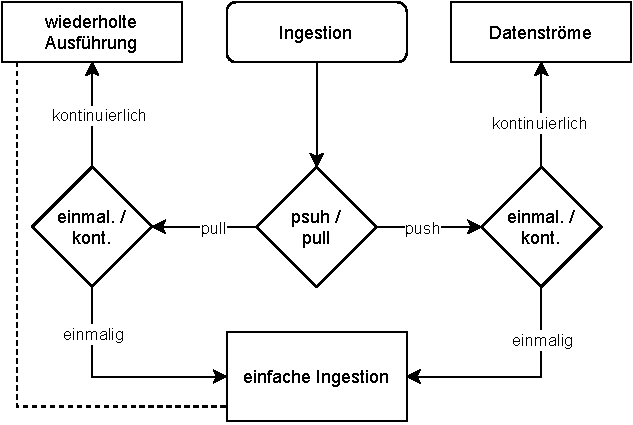
\includegraphics{ingestion-types.pdf}
    \caption{Ingestion-Typen}
    \label{fig:ingestion_types}
\end{figure}

%nochmal besser schreiben%
\subsubsection{Ingestion Start}
Als erster Schritt für die Entwicklung, muss ermittelt werden, wie der Ablauf einer Ingestion aussieht.
Dazu ist in \fref{fig:ingestion_ablauf} eine Darstellung zusehen, die mögliche Abläufe bei der Ingestion zeigt.
Es werden Abläufe unterschieden, die entweder durch einen Aufruf der API-Schnittstelle gestartet werden (blaue Pfeile) oder durch einen Trigger oder zeitgesteuert (orange Pfeile).

Der Eintrittspunkt ``API-Schnittstelle'' stellt hierbei für alle Ingestion-Typen die erste Ingestion dar.
Im darauf folgenden Verarbeitungsprozess müssen neue Metadaten erstellt werden.
Falls es sich um eine kontinuierliche Ingestion handelt, werden außerdem je nach Typ die Trigger, Zeitsteuerung oder Unterstützung für Datenströme erstellt.
Die gestrichelten Pfeile stellen dar, dass bei der wiederholten Verarbeitung der Ingestion an den entsprechenden Punkten immer wieder eingesetzt wird.
Bei der kontinuierlich-passiven Ingestion muss im Gegensatz zur aktiven nicht bei jedem Durchlauf die Ingestion-Definition neu geladen werden, da hier durchgehend auf neue Daten gewartet wird.

Bei einem Start durch kontinuierliche Ingestion fällt die Prüfung auf ein kontinuierliche Ingestion weg.
Hier kann direkt die Ingestion ausgeführt werden.
Wie genau die die Ingestion-Definition, Metadaten, Datenquellen und die Ausführung der Ingestion genau aussehen, wird später in der Arbeit behandelt.


\begin{figure}
    \centering
    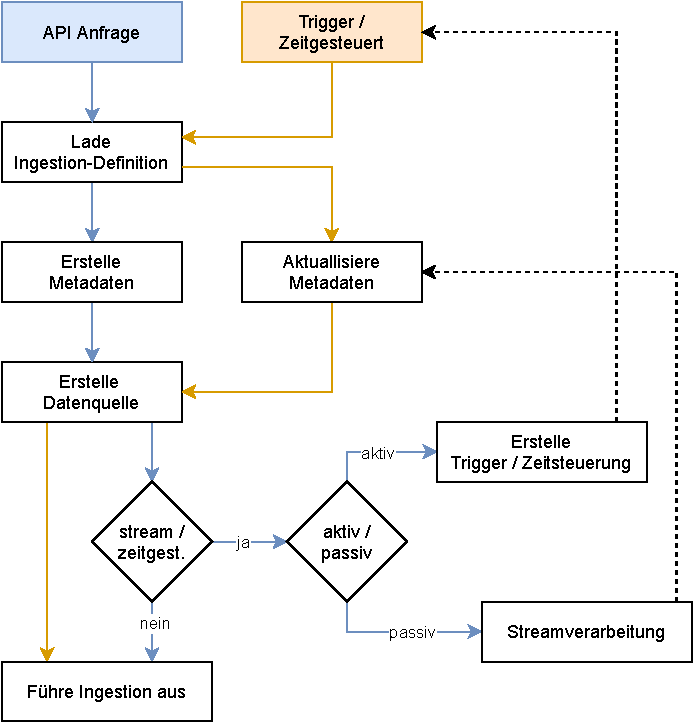
\includegraphics{ingestion-Ablauf.pdf}
    \caption{Ablauf des Starts einer Ingestion}
    \label{fig:ingestion_ablauf}
\end{figure}

\subsubsection{Ausführung Ingestion}
Die Ausführung der Ingestion sollte so entwickelt werden, dass dies unabhängig von der Datenquelle verwendet werden kann, dabei gleichzeitig so einheitlich ist wie möglich.
Dazu muss als erstes untersucht werden, an welchen Stellen der Ingestion sich die Datenquellen unterscheiden.
Da Apache Spark als Grundlage verwendet wird, ist ein Kernpunkt die Daten in ein Dataframe zu laden.
Um dieses Dataframe dann im System zu speichern, kann für jede Quelle das gleiche Vorgehen verwendet werden.

Für die Beschreibung der Datenquellen sollen hier Ingestion-Definitionen zum Einsatz kommen.
Das Ziel ist es, soviel wie Möglich von der Ingestion ohne Programmcode konfigurierbar zu machen, so dass die Benutzung des Data-Lake-Systems möglichst einfach ist.
Die Ingestion-Definition sollte alle wichtigen Informationen enthalten, die für die Ausführung einer Ingestion notwendig sind.
-- hier aufzählen --

Es gibt einige Fälle, in denen ein einfaches Laden der Daten nicht ausreicht. 
Ein Beispiel dafür ist, wenn die Daten serialisiert übertragen werden und vor dem Speichern deserialisiert werden müssen.
Um solche Szenarien zu Unterstützen sollen sogenannte Ingestion-Plugins verwendet werden.
Diese Plugins sind Code, der vordefinierte Methoden enthält, die von der Ingestion-Schnittstelle aufgerufen werden um individuelle Verarbeitung an bestimmten Stellen zu ermöglichen.
Die Liste der benötigten Plugins wird in der Ingestion-Definition mit angegeben.

\subsubsection{Server Architektur}
Der Server, der im Masterprojekt entwickelt wurde ist eine monolithische Anwendung und kümmert sich um alle Aspekte des Data Lake Systems.
Eine solche Architektur ist anfangs zwar schneller zu entwickeln, aber schwerer wartbar und die Skalierung ist nicht so einfach.
Daher soll für neue Komponenten der Mirco-Service-Ansatz verfolgt werden.
Das bedeutet, dass die Funktionen des Data-Lake-Systems auf mehrere Anwendungen verteilt werden.
Dadurch erreicht man eine Entkopplung der einzelnen Komponenten, was dazu führt, dass diese sich leichter warten und erweitern lassen.
Außerdem ist eine gezielte Skalierung bestimmter Funktionen durch Replikation einfacher und effizienter umzusetzen, da nicht eine große Anwendung sondern nur der betroffene Teil mehrfach ausgeführt werden muss.

\begin{figure}
    \centering
    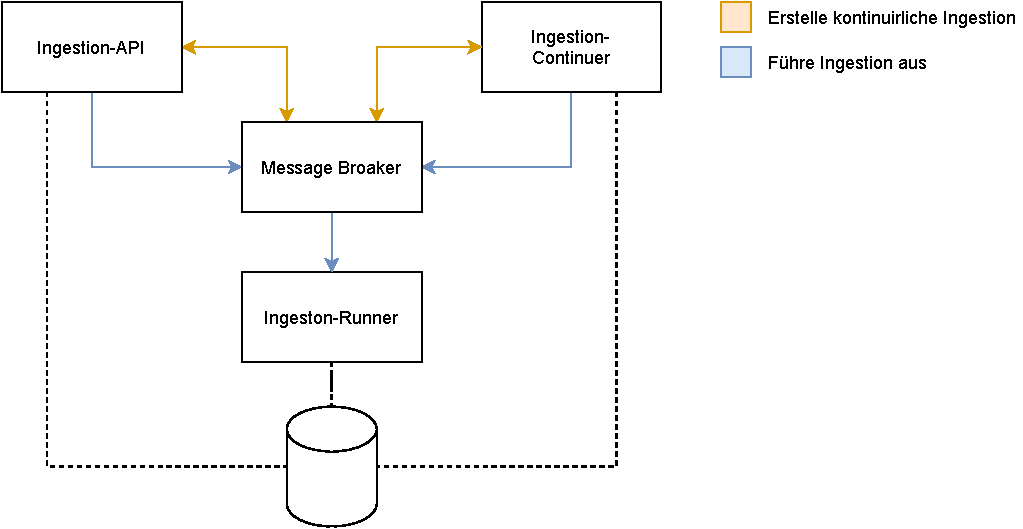
\includegraphics{ingestion-arch.pdf}
    \caption{Architektur der Ingestion Komponenten}
    \label{fig:ingestion_arch}
\end{figure}

In \fref{fig:ingestion_arch} ist zusehen, aus welchen Komponenten die Ingestion Schnittstelle zusammen gesetzt wird.
Im Zentrum steht ein System, genannt Message Broaker, das den Nachrichtenaustausch zwischen den einzelnen Komponenten verwaltet.
Die Ingestion-API stellt die REST Schnittstelle über die sowohl neue Ingestions als auch kontinuierliche gestartet werden können.
Der Ingestion-Continuer erstellt alles Nötige, damit die zeit- oder trigger-gesteuerte wiederholte Ausführung von Ingestions möglich wird.
Der Ingestion-Runner ist dafür zuständig, die einzelnen Ingestion Aufgaben auszuführen.
Zusätzlich haben alle Komponenten bis auf den Message Broaker eine Verbindung zu einer Datenbank, in der Informationen persistiert werden können.

Die API und der Ingestion-Continuer tauschen gegenseitig Nachrichten über die Erstellung aus. 
Der API Server teilt mit, was erstellt werden soll und der Continuer bestätigt, wenn die Ingestion erstellt wurde, damit die API die entsprechende Schnittstelle bereitstellen kann.
Außerdem startet der Continuer die zeitgesteuerten Ingestions.
Beide Komponenten versenden außerdem Nachrichten zur Ausführung einer Ingestion.
Die Nachrichten zur Ausführung einer Ingestion werden an einen Ingestion-Runner gesendet, der diese Ingestion dann ausführt.
Es kann im Data Lake System mehrere Ingestors geben, um viele gleichzeitige Ingestions zu ermöglichen.

\subsection{Plugins}
Da Daten nicht immer einfach aus einer Daten-Quelle geladen werden können, sollte es eine Möglichkeit geben, den Code des Servers dynamisch zu erweitern.
Als Lösung dafür werden Plugins verwendet.
Plugins sind extra Code, der eine vordefinierte Form haben muss und an bestimmten stellen der Ingestion ausgeführt werden kann.
Für jede neue Ingestion sollte es möglich sein Plugins hinzuzufügen.
Ein Plugin kann eine oder mehrere Methoden implementieren, die bestimmen, wann der Code in der Ingestion ausgeführt wird.
\begin{itemize}
    \item load(SparkSession): Dataframe\\
    Die load-Methode ersetzt das standard Verhalten der Ingestion beim Laden der Daten. 
    Diese Methode erhält die SparkSession und muss ein Dataframe mit den Daten zurück liefern.
    \item after\_load(Dataframe): Dataframe \\ 
    after\_load() kann Implementiert werden, um das Dataframe nach dem Laden und vor der Metadatenextraktion zu manipulieren.
    \item get\_metadata(Dataframe): Dict \\
    Mit dieser Methode können extra Metadaten aus dem Dataframe extrahiert werden.
\end{itemize}

\subsubsection{REST Schnittstelle}
In diesem Abschnitt wird das Design der REST API besprochen.
Da die Inegstion-Schnittstelle generisch sein soll, werden alle Quellen spezifischen Einstellungen über Parameter an den Server gegeben.
Dazu gehören: 
\begin{itemize}
    \item jars: Extra Abhängigkeiten die über \textit{Maven}\footnote{https://maven.apache.org/} geladen werden.
    \item format: Zu lesendes Format der Daten.
    \item options: Options werden der read-Methode von \textit{PySpark} mit gegeben und können zum Beispiel den Host oder Port einer Datenbank enthalten.
    Welche Options genau zur Verfügung stehen, hängt davon ab, welches Format und welche Jars für das Laden genutzt werden.
    \item plugins: Liste von Benutzerdefinierten Plugins, die wärend der Ingestion verwendet werden sollen.
\end{itemize}

Für die einwickelte Architektur werden die nachfolgenden Endpunkte für die REST API benötigt.
\paragraph{/api/v2/ingestion - POST}
Über diesen Endpunkt sollen Datenquellen hinzugefügt und Ingestions gestartet werden können.

\begin{description}
    \item[/api/v2/ingestion] 
    \item Abfrage der Ingestions
    \item Trigger für wiederholte Ausführung
\end{description}